\documentclass[journal,12pt,twocolumn]{IEEEtran}
\usepackage[top = 0.9in,bottom = 0.9in,left = 0.8in,right = 0.8in]{geometry}
\setlength{\columnsep}{1cm}
\usepackage{amssymb}
\usepackage{amsfonts}
\usepackage{amsmath}
\usepackage{amsthm}
\usepackage{setspace}
\usepackage{longtable}
\usepackage{enumitem}
\usepackage{mathtools}
\usepackage{color}                                  
\usepackage{array}
\usepackage{calc} 
\usepackage{bm}
\usepackage{caption}
%to remove 'table 1'
\usepackage{float}
%to fix position (H)
\setlength{\parindent}{0pt}
%no indentation for paragraphs


\newcommand{\rectarea}[2]{#1 \times #2}  
% area of rectangle
\newcommand{\cirarea}[1]{\pi \times (#1)^2} 
% area of circle
\newcommand{\semicirarea}[1]{\frac{1}{2} \times \pi \times (#1)^2} 
% area of semicircle
\newcommand{\quatercirarea}[1]{\frac{1}{4} \times \pi \times (#1)^2} 
% area of quarter circle


\begin{document}

\title{ASSIGNMENT-1}
\author{Mukunda Reddy AI21BTECH11021}
\date{}
\maketitle

\section*{\large Question 3(c)}
\begin{figure}[H]
    \centering
    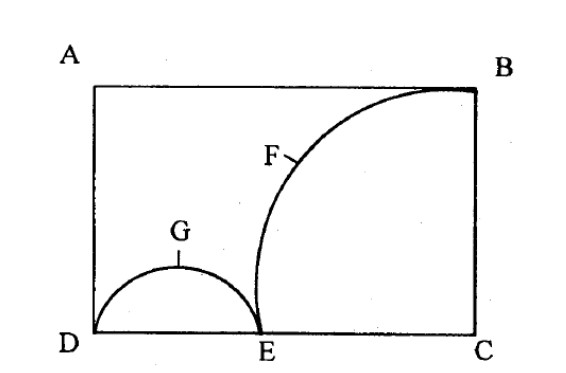
\includegraphics[scale = 0.5]{Figure_1.jpg}
\end{figure}

In the figure given below, ABCD is a rectangle.${AB = 14cm}$ and
${BC= 7 cm}$.From the rectangle, a quarter circle BFEC and a
semicircle DGE are removed.Calculate the area of the remaining
piece of the rectangle?.\\
( Take $ \pi = 22/7 $)\\
\hline
\section*{\underline{\Large{Solution\:}}}

\begin{table}[H]
    \centering
    \renewcommand{\arraystretch}{1.5}
    \begin{tabular}{|c|p{1.5cm}|p{1.2cm}|p{1.2cm}|}
    \hline
    Shape & Rectangle & semi circle & Quarter circle\\ \hline
    Area &$l*b$ & $\frac{1}{2}\pi r^2$ & $\frac{1}{4}\pi r^2$\\
    \hline
    \end{tabular}
    \caption*{Areas of various shapes}
\end{table}

\begin{center}
 \begin{align*}
    \text{so area of rectangle ABCD}&= \rectarea{l}{b} \\
                 &= \rectarea{14cm}{7cm} \\
                 &= 98cm^2.\\
  \end{align*}
\end{center}
\columnbreak

  \begin{center}
  \begin{align*}
        \text{since BC and EC are the radius of same} circle&\\
    \implies \text{The length of} BC = EC = 7cm.&\\
        \text{since AB and DC are the radius of same circle&}\\
    \implies \text{length& of}AB = DC = 14cm.& \\ 
                     \text{So}\ DE=DC-EC =7cm.& \\ 
\therefore \text{The radius of semicircle GDE} =\frac{DE}{2}=\frac{7}{2}cm&\\
 \end{align*}
    \end{center}
  
\begin{align*}
\text{Area of BFEC region} &= \quatercirarea{r} \\
&= \frac{1}{4} \times \pi \times 7cm \times 7cm\\ 
               &= \frac{77}{2}cm^2.\text{(radius is BC)}\\
\end{align*}

\begin{align*}
\text{Area of GDE region} &= \semicirarea{r} \\
               &=\frac{1}{2} \times \pi \times \frac{7}{2}cm \times \frac{7}{2}cm.\\
                          &= \frac{77}{4}cm^2.\\
\end{align*}
      
To get the area of the remaining part take total are of rectangle
and subtract the areas of semicircle and quarter circle.
\begin{align*}
    \text{Required area} &= \rectarea{14cm}{7cm} \\
                     &- \semicirarea{7cm} - \quatercirarea{\frac{7}{2}} \\
\end{align*}

   
\begin{align*}
\implies area required &=98cm^{2} - \frac{77}{2}cm^{2} - \frac{77}{4}cm^{2}\\ 
&= \frac{161}{4}cm^{2} \\
&= 40.25cm^{2}  \\
    \end{align*}

\begin{center}
\renewcommand{\arraystretch}{1.1}
\begin{tabular}{|c|}
\hline
    $$ \therefore \text{Area of the remaining piece of rectangle} = 40.25cm^2 $$ &\\
\hline
\end{tabular}
\end{center}

\begin{figure}
    \centering
    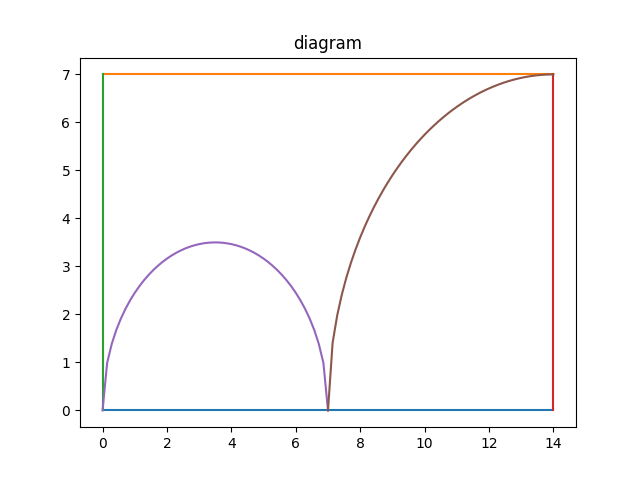
\includegraphics[scale = 0.6]{Figure_2.png}
    \caption{python graph}
    \label{fig:my_pythondiagram}
\end{figure}

\begin{figure}
\begin{center}
\textbf{Verification in python}    
\end{center}
    \centering
    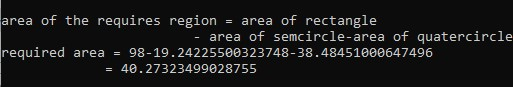
\includegraphics[scale = 0.75]{Figure_3.jpg}
    \caption{python code}
    \label{fig:my_codeverification}
\end{figure}

\end{document}
